%\documentclass[final,hyperref={pdfpagelabels=false}]{beamer}
\pdfminorversion=4
\documentclass[xcolor=dvipsnames]{beamer}



%Load the myriad packages
\usepackage{xcolor}
\usepackage{subcaption}
\usepackage{tikz}
\usetikzlibrary{shapes.geometric, arrows}
\tikzstyle{startstop} = [rectangle, rounded corners, minimum width=2cm, text
    width=1.8cm, minimum height=1cm,text centered, text=white,draw=black, fill=Gray!140]
\tikzstyle{io} = [trapezium, trapezium left angle=70, trapezium right angle=110,
minimum width=0.5cm, minimum height=1cm, text centered, draw=black,
fill=blue!20!Gray!90!,text=white]
\tikzstyle{process} = [rectangle, minimum width=2cm, minimum height=1cm, text
centered, text width=2cm, draw=black, text=white,fill=Gray!140!blue!70!white]
\tikzstyle{decision} = [diamond, minimum width=2.0cm, minimum
    height=0.81cm,aspect=1.40, text centered, draw=black, fill=Gray!,text=white]
\tikzstyle{arrow} = [thick,line width=0.5mm,->,>=stealth]
\tikzstyle{arrow1} = [dashed,->,>=stealth]

%Math commands
\newcommand{\deriv}[2]{\frac{\mathrm{d} #1}{\mathrm{d} #2}}
\newcommand{\pderiv}[2]{\frac{\partial #1}{\partial #2}}
\newcommand{\bx}{\mathbf{X}}
\newcommand{\ba}{\mathbf{A}}
\newcommand{\by}{\mathbf{Y}}
\newcommand{\bj}{\mathbf{J}}
\newcommand{\bs}{\mathbf{s}}
\newcommand{\B}[1]{\ensuremath{\mathbf{#1}}}
\newcommand{\Dt}{\Delta t}
\renewcommand{\d}{\mathsf{d}}
\newcommand{\mom}[1]{\langle #1 \rangle}
\newcommand{\xl}{{x_{i-1/2}}}
\newcommand{\xr}{{x_{i+1/2}}}
\newcommand{\il}{{i-1/2}}
\newcommand{\ir}{{i+1/2}}

%other commands
\renewcommand{\u}[1]{\underline{#1}}
\newcommand{\iso}[2]{${}^{{#2}}${#1} }
\newcommand{\nubar}[0]{$\overline{\nu}$ }
\newcommand{\expect}[1]{E[#1] }
\newcommand{\colg}[1]{{\color{ForestGreen} #1}}
\newcommand{\coly}[1]{{\color{yellow} #1}}
\newcommand{\colw}[1]{{\color{white} #1}}
\newcommand{\colb}[1]{{\color{blue} #1}}
\newcommand{\colr}[1]{{\color{red} #1}}

\usepackage{amssymb,amsmath}
\usepackage[english]{babel}
\usepackage[latin1]{inputenc}
\usepackage[orientation=portrait,size=a0,scale=1.4]{beamerposter}
\usepackage{textcomp}
\usepackage{graphicx}
%\usepackage{tikz}
%\usepackage[numbers, super]{natbib}
\usepackage{grffile} %spaces in file names
\usepackage{parskip}
%\usepackage[T1]{fontenc} %for sc and bf
%\usepackage{times}
\usepackage{wasysym}
\usepackage{bigstrut}
\usepackage{float}
\usepackage{setspace}
%\usepackage{enumitem}
%\setlist{nolistsep} % or \setlist{noitemsep} to leave space around whole list
% Load some optional sub-parts of PGF
%\usetikzlibrary{decorations.pathmorphing}
%\usetikzlibrary{positioning}
%\usetikzlibrary{calc}
%\usetikzlibrary{shapes.geometric}
%\usepackage{pgfplots}

%misc.
\newcommand{\nn}[1]{\ensuremath{^{#1}}} %[1] is # of commands
\newcommand{\keff}{\ensuremath{{k_\mathrm{eff}}}}
\newcommand{\kinf}{\ensuremath{{k_\infty}}}
\newcommand{\alphaT}{\ensuremath{{\alpha_{_T}}}}
\newcommand{\SN}{\ensuremath{{\text{S}_\text{N}}}}
%Note: tarticle has ``several'' changes from article
%in this vein.
% some simplifying commands

\newcommand{\eg}{{\it e.g.}}
\newcommand{\ie}{{\it i.e.}}
\newcommand{\etal}{{\it et al.\,}}
\newcommand{\acite}[1]{{\bf(Add Citation: #1)}}
\newcommand{\E}{\mathcal{E}}
% derivative - d
\newcommand{\ud}{\,\mathrm{d}}
% bold unit vector n-hat
\newcommand{\nhat}{\hat{\bf n}}
\newcommand{\tensor}[1]{\mathcal{#1}}
\renewcommand{\vec}[1]{\mathbf{#1}}
\newcommand{\om}{\boldsymbol{\Omega}}
%

\graphicspath{{../images/}}
%\listfiles
%\boldmath

%%%%%%%%%%%%%%%%%%%%%%%%%%%%%%%%%%%%%%%%%%%%%%%%%%%%%%%%%%%%%%%
% Optional packages, used to show off certain tricks

\newlength \figwidth
\setlength \figwidth {0.5\textwidth}

%%%%%%%%%%%%%%%%%%%%%%%%%%%%%%%%%%%%%%%%%%%%%%%%%%%%%%%%%%%%%%%

\mode<presentation>
{
   \usetheme{TAMU}
}

\title{\color{black}A High-Order Low-Order Algorithm with Exponentially Convergent Monte Carlo for Thermal Radiative Transfer}

\author{\large Simon~R.~Bolding \& Jim~E.~Morel}

%TAMU
\institute{Department of Nuclear Engineering,
Texas A\&M University -- CERT Project}

% You can override the default acknowledgment, and address if you want
%\acknowledgement{*Submitted in partial fulfillment of the requirements of NUEN 610 \\
%(Nuclear Reactor Design)}
%\address{Nuclear Engineering Department \\
%            Texas A\&M University \\
%            College Station, TX 77843-3133}}

% If you don't want the menu section outline above the title, do this:
%\setbeamertemplate{headline}{}

\newlength{\columnheight}
\setlength{\columnheight}{105cm}

%%%%%%%%%%%%%%%%%%%%%%%%%%%%%%%%%%%%%%%%%%%%%%%%%%%%%%%%%%%%%%%%%%%%%%%%%%%%%%%%%%%%%%%%%%%%%
\begin{document}
\begin{frame}
\begin{columns}

    % ---------------------------------------------------------%
    % Set up a column
\begin{column}{.49\textwidth}
\begin{beamercolorbox}[center,wd=\textwidth]{postercolumn}
\begin{minipage}[T]{0.95\textwidth} % tweaks the width, makes a new \textwidth
\parbox[t][\columnheight]{\textwidth}{ % must be some better way to set the the height, width and textwidth simultaneously
         % Since all columns are the same length, it is all nice and tidy.  You have to get the height empirically
         %%%%%%%%%%%%%%%%%%%%%%%%%%%%%%%%%%%%%%%%%%%%%%%%%
       \begin{block}{Background on Thermal Radiative Transfer}
         \begin{itemize}
             \setlength{\itemsep}{0.6em}
             \item The continuous radiation and material energy
                 equations are
\begin{align}
    \frac{1}{c}\pderiv{I}{t} + \mu \pderiv{I}{x} + \sigma_t I(x,\mu,t)
    &= \frac{\sigma_s \phi(x)}{4\pi} +  \frac{1}{4\pi} \sigma_a a c T^4,\label{ho_trans}
  \\
  C_v \pderiv{T(x,t)}{t} &=  {\sigma_a \phi(x,t)} - {\sigma_a a c T^4} \label{lo_mat}
\end{align}
     \item The radiation intensity $I(x,\mu,t)$ and material temperature
         $T(x,t)$ are
         \textbf{coupled}
         through photon \textbf{emission} $\sigma_a a c T^4$ and
         \textbf{absorption} $\sigma_a \phi$.
      \item We form a \textbf{lower-dimensional} system which can
          efficiently \textbf{resolve non-linearities} in the problem.  The low-order
          (LO) equations contain consistency terms that preserve accuracy
          of \textbf{efficient}, high-order (HO) Monte Carlo simulations.
      \item We recently have included the time variable in the Monte Carlo transport algorithm,
          improving accuracy in optically thin problems.
      \end{itemize}
         \end{block}
         \vfill
         %%%%%%%%%%%%%%%%%%%%%%%%%%%%%%%%%%%%%%%%%%%%%%%%%
	\begin{block}{Algorithm}
        \resizebox{0.9618\linewidth}{!}{
    \fontsize{10}{11.0}\selectfont
    \begin{tikzpicture}[node distance=2cm]
        \node (start) [startstop] {Initialize LO system with $I^n$};
        \node (in1) [process, right of=start, xshift=2cm, text width=3.3cm]  {{(A)}
        \colw{LO Newton solve, fully converged}};%{LO solve:\vspace{0.041in}        $\B D(\mu^{HO})\Phi = \frac{1}{\keff}\B F\Phi$};
        \node (pro1) [io, below of=in1] {$T_{LD}^{n+1}(x)$, $\phi_{LD}^{n+1}(x)$};
        \node (dec1) [decision, below of=pro1, yshift=-0.5cm, text width=1.74cm] {Outer Converged?};
        \node (pro2a) [process, left of=dec1, xshift=-2.0cm] {Move to the next time step};
        \node (srcs) [process, right of=dec1, xshift=3.0cm, text width=2.8cm] {{{(B)}}
        \colw{Construct LD emission source}};
        \node (pro2b) [process, above of=srcs, yshift=0.5cm] {{(C)} \colw{HO solve
        for $\tilde I^{n+1}(x,\mu)$}};
        \node (cons) [process, above of=pro2b, text width=3.0cm] {{(D)} \colw{Compute consistency
        terms}};
        \draw [arrow1] (start) -- (in1);
        \draw [arrow] (in1) -- (pro1);
        \draw [arrow] (pro1) -- (dec1);
        \draw [arrow] (srcs) -- (pro2b);
        \draw [arrow] (dec1.east) -- node[anchor=south] {no} (srcs);
        \draw [arrow1] (dec1.west) -- node[anchor=south] {yes} (pro2a);
        \draw [arrow1] (pro2a) -- (start);
        \draw [arrow] (pro2b) -- (cons);
        \draw [arrow] (cons) -- (in1);
    \end{tikzpicture}
}
	\end{block}
	\vfill
         \vfill
         %%%%%%%%%%%%%%%%%%%%%%%%%%%%%%%%%%%%%%%%%%%%%%%%%%%%%%%%%
         \begin{block}{Details of the algorithm} 
         \setlength\itemsep{0.2em}
            \begin{itemize}
                \item[{(A)}] The LO equations are formed by taking spatial, angular, and temporal
                    moments of Eq.~\eqref{ho_trans} \& ~\eqref{lo_mat},
                    defined locally over the $i$-th spatial finite element (FE). \vspace{0.2em}
        \end{itemize}
       \begin{minipage}{0.45\textwidth}
        \centering
        \resizebox{0.99\linewidth}{!}{
            {\tiny
                \begin{tikzpicture}[scale=1.3]
 %                   \node at (3.2105,6.00) {\tiny \colb{Spatial Element $i$}};
                    \draw (0.8,5.0) -- (1.2,5.0) node[anchor=east]{$1$ \hspace{0.4em} };
            \draw (1.0,0.4) -- (1.0,0.6) node[below, pos=0.4] {$x_{i-1/2}$};
            \draw (5.90,0.4) -- (5.90,0.6) node[below, pos=0.4] {$x_{i+1/2}$};
            \node at (4.8,5.0) {$b_{R,i}(x)$};
            \node at (2.0,5.0) {$b_{L,i}(x)$};
            \draw [thick,->] (-0.5,0.5) -- (7.0,0.5) node[anchor=north west] {$x$};
            \draw [dashed,->] (5.90,0.5) -- (5.90,5);
            \draw [dashed,->] (1.0,0.5) -- (1.0,5.5);
            \draw (1.0,0.5) -- (5.90,5.0);
            \draw (5.90,0.5) -- (1.0,5.0);
        \end{tikzpicture}
    }
}
%       \begin{figure}
%    \begin{centering}
%        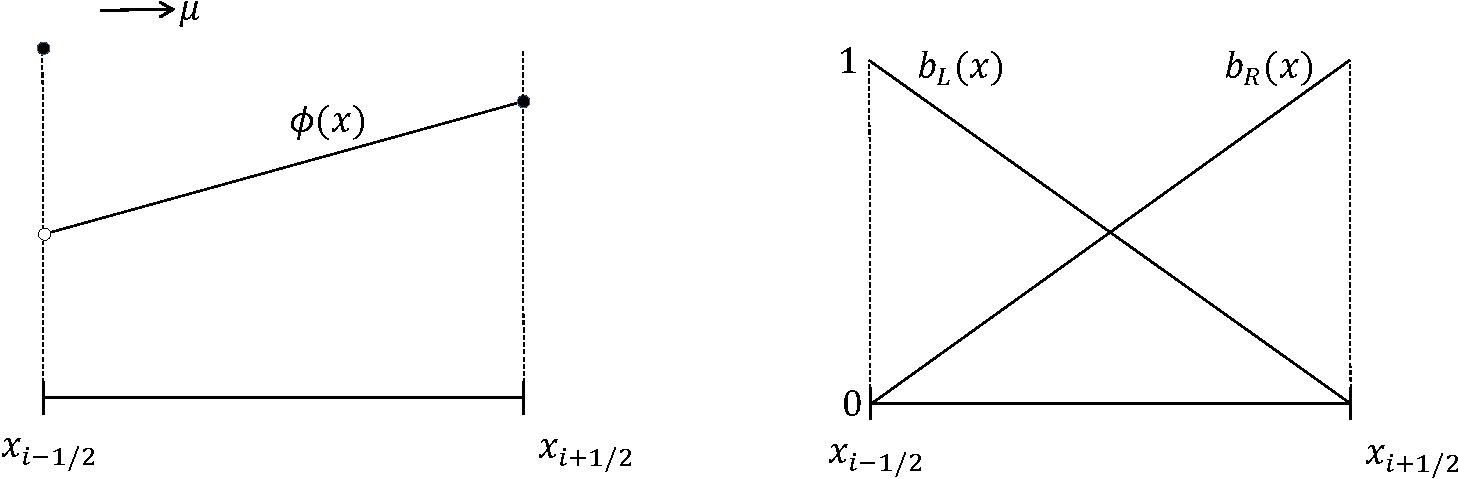
\includegraphics[trim=5.0in 0.0in 0.0in 0.0in,clip,width=0.9\textwidth]{LD.pdf}
%    \end{centering}
%    \end{figure}
    \end{minipage}
    \begin{minipage}{0.45\textwidth}
    \begin{center}
        {\small
    \begin{tabular}{c}
        \underline{Spatial moments} \\[1em]
        $ {\displaystyle \mom{\cdot}_{L/R,i} = \frac{2}{h_i} \int_{x_\il}^{x_\ir}
        b_{L/R,i}(x)(\cdot) \d x \quad }$  \\[1em]  \underline{Angular half-ranges}
        \\[1em] ${ \quad \displaystyle \phi^\pm(x) =
        \pm\int_0^{\pm 1} I(x,\mu) \d \mu}$
\end{tabular}}
    \end{center}
\end{minipage}
    \begin{itemize} 
        \setlength\itemsep{0.5em}
        \item[] Based on the current HO estimate of consistency terms,
        the non-linearities in $T$ are fully resolved \emph{for each LO solve}, using \colb{Newton's
method.}    
        \item[(B)] The HO emission source is constructed from the previous LO
            solution, producing a \textbf{fixed source,
            pure absorber} HO
            problem. 
        \item[(C)] \emph{For each HO solve}, multiple exponentially-convergent Monte
            Carlo (ECMC) batches are performed to solve a pure absorber transport problem. 
            \begin{itemize}
        \setlength\itemsep{0.5em}
            \vspace{0.46em}
        \item  Each ECMC batch \colb{tallies the error} in the latest estimate of the solution.
        By initializing the first estimate of $\tilde I^{n+1}$ to $\tilde I^{n}$, \textbf{very few histories are
            needed} because we are only estimating the change in $I$ over a time
            step.
        \item ECMC uses a
            \textbf{projection of the exact solution} onto a linear
            discontinuous (LD) finite element, \colb{space-angle} mesh
            denoted $\tilde{I}^{n+1}$.
        \end{itemize}
    \item[(D)] We use the latest ECMC solution for $\tilde{I}^{n+1}$ to evaluate
        \colb{angular consistency terms} in the LO equation, e.g.,
        \begin{equation*}
            \overline{\mu}^+_L = \frac{\mom{\mu\, I^{HO}}_L^+}{\mom{I^{HO}}_L^+}
        \end{equation*}
\end{itemize}
\end{block}
%%%%%%%%%%%%%%%%%%%%%%%%%%%%%%%%%%%%%%%%%%%%%%%%%%%%%%%%%
\begin{block}{Diffusion Synthetic Acceleration (DSA) of LO equations} 
\setlength\itemsep{0.2em}
   \begin{itemize}
       \item We perform DSA-accelerated source iterations on the effective scattering source resulting from linearization of the LO equations. 
       \item A spatially \colb{continuous} discretization of the diffusion equation is applied to the residual equation for scattering iterations.  The estimated error is mapped onto the 
       moment unknowns based on a \colb{discontinuous} discretization of the P$_1$ equations over each cell. 
         \item In a modified version of the two material problem, DSA \textbf{reduced
             the spectral radius of iterations from 0.993 to $<$0.1.}
   \end{itemize}
\end{block}
\vfill
%%%%%%%%%%%%%%%%%%%%%%%%%%%%%%%%%%%%%%%%%%%%%%%%%%%%%%%%%%%%%
}
\end{minipage}
\end{beamercolorbox}
\end{column}
\begin{column}{.49\textwidth}
\begin{beamercolorbox}[center,wd=\textwidth]{postercolumn}
\begin{minipage}[T]{0.95\textwidth} % tweaks the width, makes a new \textwidth
\parbox[t][\columnheight]{\textwidth}{ % must be some better way to set the the height, width and textwidth simultaneously
         % Since all columns are the same length, it is all nice and tidy.  You have to get the height empirically
    %%%%%%%%%%%%%%%%%%%%%%%%%%%%%%%%%%%%%%%%%%%%%%%%%
    %%%%%%%%%%%%%%%%%%%%%%%%%%%%%%%%%%%%%%%%%%%%%%%%%
 %   \begin{columns}
 %       \column{0.015\textwidth}
 %       \column{0.47\textwidth}
        %
 %       \begin{block}{High-fidelity weighting function}
 %       \centering
 %       %\includegraphics[width=\figwidth]{../results/images/p1/e1/refWgt/base/p_effsigt.pdf} \\
 %       {\small Region-averaged reference solution} \\
 %       \end{block}
 %       %
 %       \column{0.025\textwidth}
 %       \column{0.47\textwidth}
 %       \begin{block}{Low-fidelity weighting function}
 %       \centering
 %       %\includegraphics[width=\figwidth]{../results/images/p1/e1/NJOYwgt/base/p_effsigt.pdf} \\
 %       {\small Essentially $1/E$} \\
 %       \end{block}
 %   \end{columns}
 %   \vfill
 %   %%%%%%%%%%%%%%%%%%%%%%%%%%%%%%%%%%%%%%%%%%%%%%%%%
 %  \begin{block}{ Better accuracy per DOF than standard MG}
 %     \centering
 %  \vspace{-3mm}
 %   Problem 4, Base problem, Errors in QOI
 %   \vspace{3mm}
 %   \begin{columns}[b]
 %   %
 %   \column{0.5\textwidth}
 %   \centering
 %   {\small Reference weighting }
 %   %\includegraphics[width=\figwidth]{../results/images/p4/e4/refWgt/base/p_common_err.pdf} \\
 %   %\includegraphics[width=\figwidth]{../results/images/p4/e4/refWgt/resonanceRes/p_common_res_k-eig.pdf} \\
 %   %
 %   \column{0.5\textwidth}
 %   \centering
 %   {\small Generic weighting }
 %   %\includegraphics[width=\figwidth]{../results/images/p4/e4/NJOYwgt/base/p_common_err.pdf} \\
 %   %\includegraphics[width=\figwidth]{../results/images/p4/e4/NJOYwgt/resonanceRes/p_common_res_k-eig.pdf} \\
 %   \end{columns}
 %   \end{block}
    \begin{block}{Results for two Marshak wave test problems}
    \begin{itemize}
        \setlength\itemsep{0.2em}
        \item For all HOLO results only one outer iteration is performed, per time
            step. Figures depict radiation temperature $T_R = \sqrt[4]{\phi/(ac)}$.
    \end{itemize}
    \vspace{0.7em}
    \centering \textbf{Two Material Problem:} Optically thin (left) and thick (right) regions
\begin{figure}
\begin{subfigure}{0.49\textwidth}
    \centering
    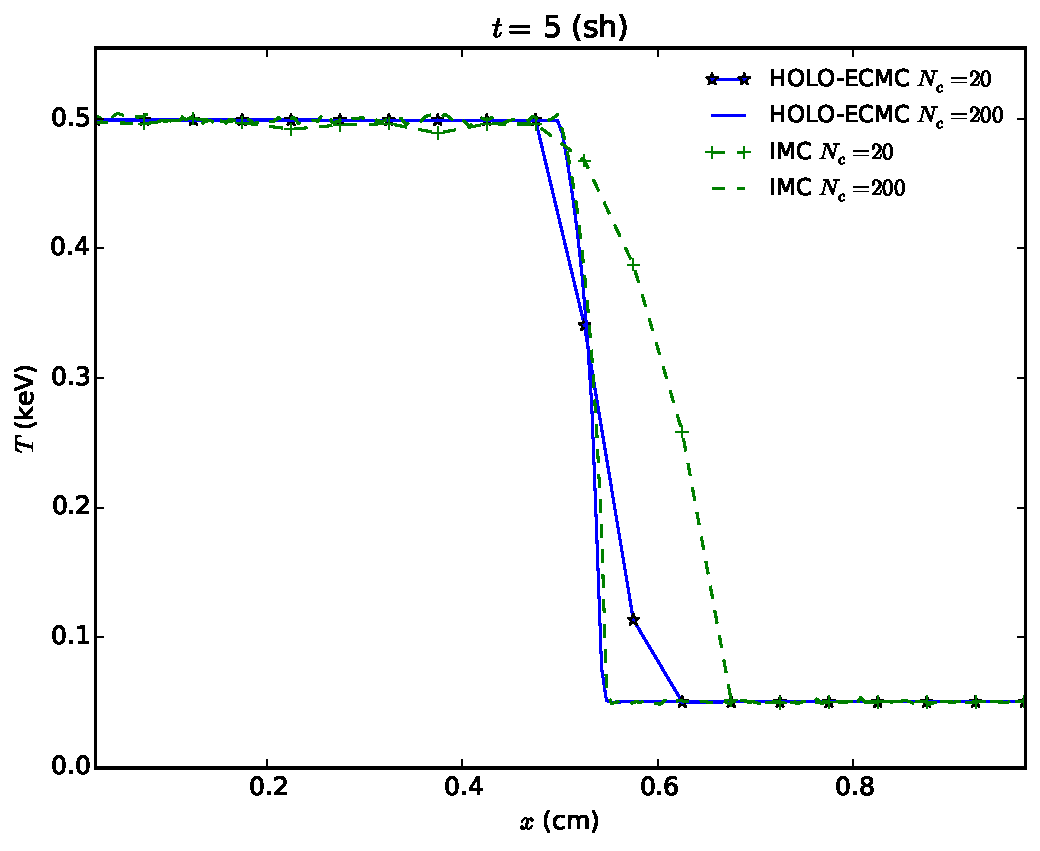
\includegraphics[width=0.99\textwidth]{two_mat_conv.pdf}
    \caption{Spatial mesh convergence.\label{twomat_full}}
\end{subfigure} 
\begin{subfigure}{0.49\textwidth}
\centering
    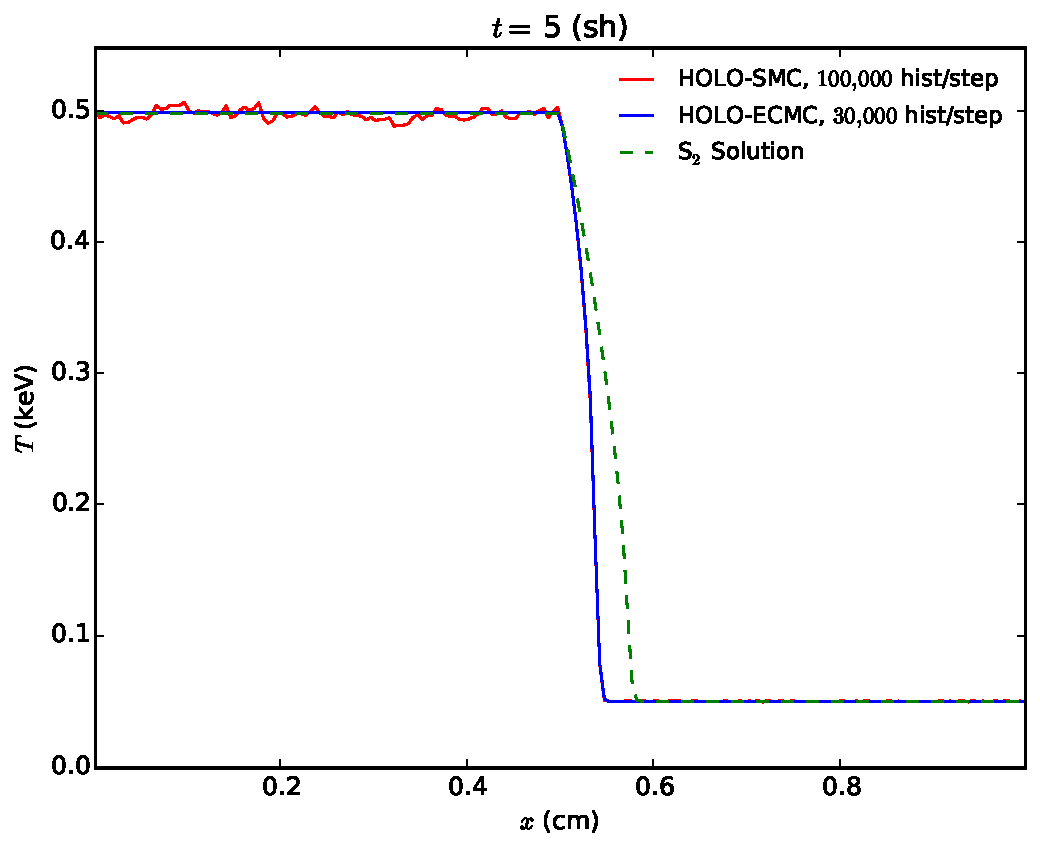
\includegraphics[width=0.99\textwidth]{two_mat_ho_compare.pdf}
    \caption{\colb{ECMC} vs \colr{Standard MC} as HO solver \label{twomat_quick}}
\end{subfigure}
\end{figure}
    \vspace{1.5em}
\centering \textbf{Equilibrium Diffusion Limit Problem}: large $\sigma_a$ and small $C_v$.
\begin{figure}
    \begin{subfigure}{0.99\textwidth}
  \centering
    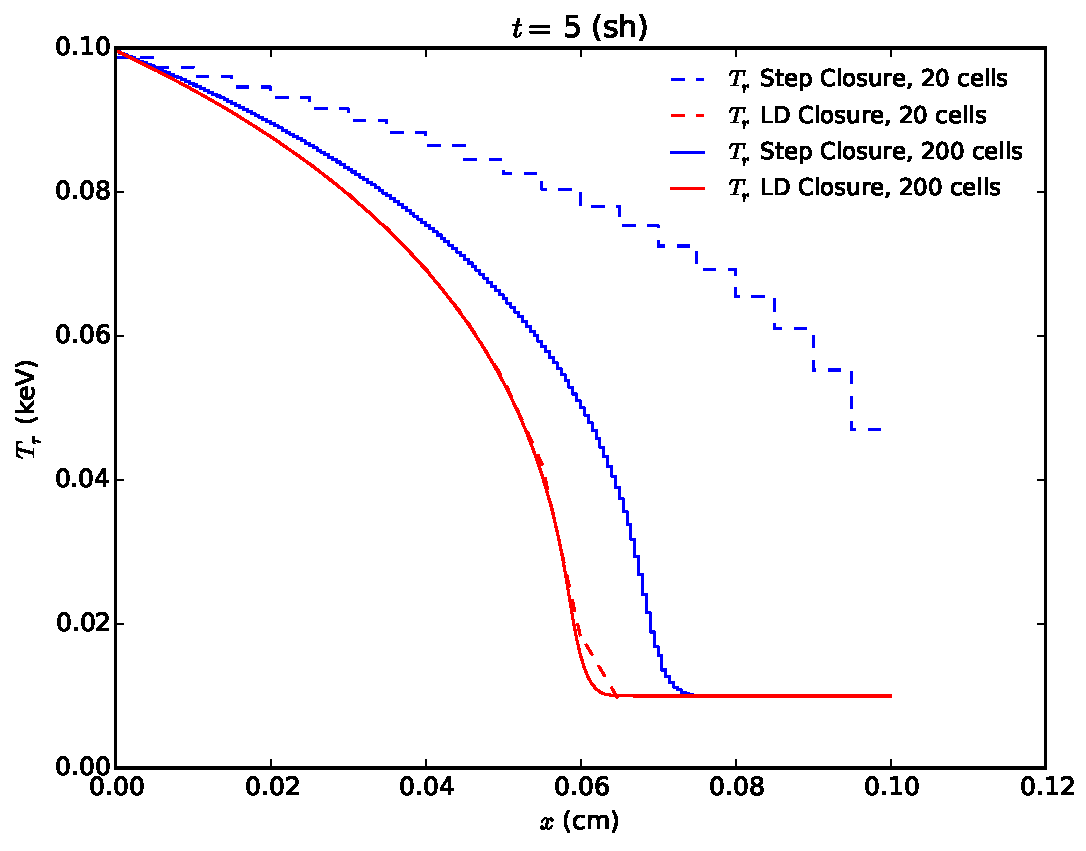
\includegraphics[width=0.49\linewidth]{diff_limit_compare.pdf}
\caption{\label{diff_limit_compare}Comparison of HOLO using LD and step discretizations in LO equations.}
  \end{subfigure}
\end{figure}
    \end{block}
    \vfill
    %%%%%%%%%%%%%%%%%%%%%%%%%%%%%%%%%%%%%%%%%%%%%%%%%
     %%%%%%%%%%%%%%%%%%%%%%%%%%%%%%%%%%%%%%%%%%%%%%%%%%%%%%%%%%%%%%%%%%%%%%%%%%%%%%%%
    \vfill
    \vfill
    \begin{block}{A fixup is necessary near strong solution gradients}
        \begin{itemize}
        \setlength\itemsep{0.5em}
            \item In strongly absorbing regions, the linear discontinuous spatial
                representation can lead to \colr{unphysical negative solutions} in certain cells
            \item In the LO system,  we set a strict floor value and preserve energy
                conservation to determine the cell average.
            \item For the HO system, we \textbf{rotate} $\tilde{I}(x,\mu)$ to be strictly positive after
                each batch. However, $\tilde{I}_{\text{rotated}}(x,\mu)$ doesn't satisfy
                the original residual equation, so the ECMC convergence quickly
                \colr{stagnates}.  Thus, we add an artifical source
                $\tilde\delta(x,\mu)$, which is 
                estimated \emph{iteratively} as
                \begin{equation*}
                    \tilde\delta(x,\mu) = \mathbf{L}(\tilde{I}^{n+1} -
                    \tilde{I}^{n+1}_{\text{rotated}})
                \end{equation*}
                where $\mathbf{L}$ is the continuous streaming plus removal operator. The solution will now converge 
                towards the \colb{strictly positive} projection $\tilde{I}_{\text{rotated}}^{n+1}$.
            \item We also allow the outflow from the cell to be \textbf{discontinuous}, allowing for greater angular accuracy on faces
                \begin{figure}[H]
                \centering
                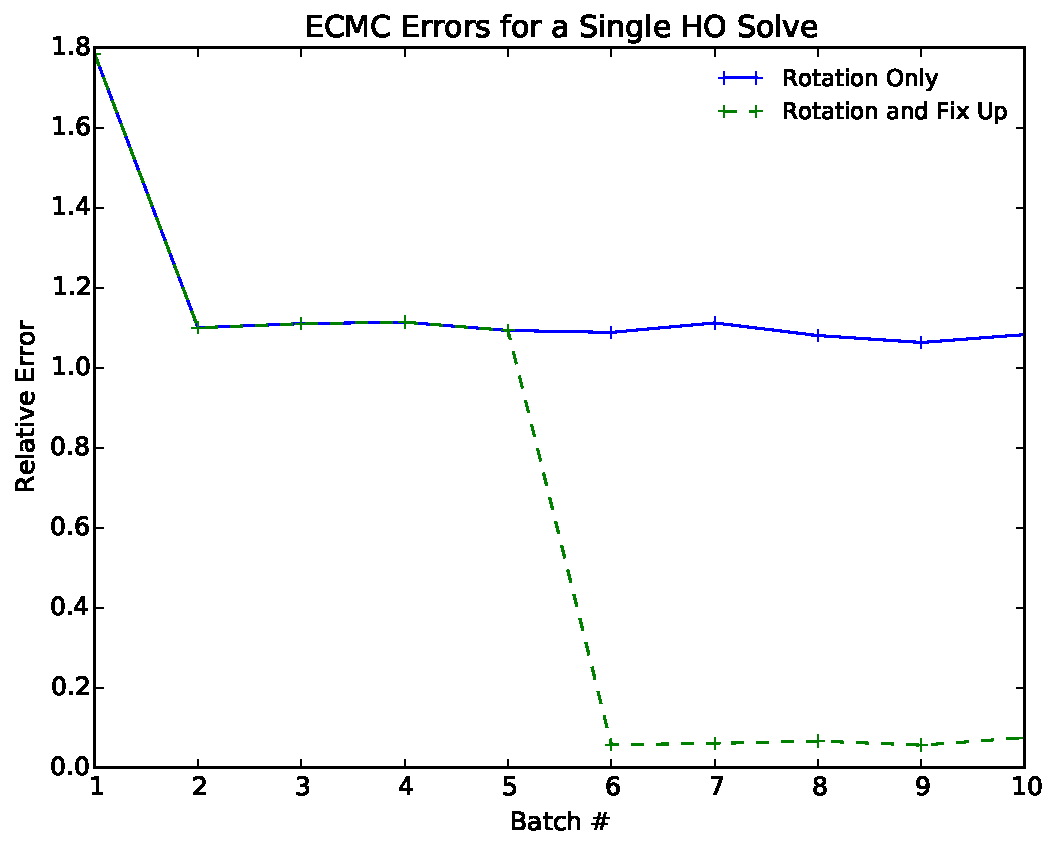
\includegraphics[width=0.5\textwidth]{errors.pdf}
             \end{figure}
        \end{itemize}
    \end{block}

    %%%%%%%%%%%%%%%%%%%%%%%%%%%%%%%%%%%%%%%%%%%%%%%%%
     \vfill
    %%%%%%%%%%%%%%%%%%%%%%%%%%%%%%%%%%%%%%%%%%%%%%%%%
    \begin{block}{Ongoing work}
    \begin{itemize}
        \setlength\itemsep{0.25em}
        \item We are working towards a \colb{linear-discontinuous} trial space in time.  ECMC will be used to estimate
              the slope of the intensity in time, which can be used to extrapolate to the end of the time step.  This  
              representation will improve the statistical efficiency of tallies used to estimate $\tilde I(x,\mu)$ at 
              the end of the time step because all particles contribute to the local slope
        \item The LD time space will require a different sampling approach, which will be useful to investigate for extending
              ECMC to higher spatial dimensions.
        \end{itemize}
    \end{block}
     \vfill
    \begin{block}{Acknowledgements}
        \begin{figure}
            \centering
            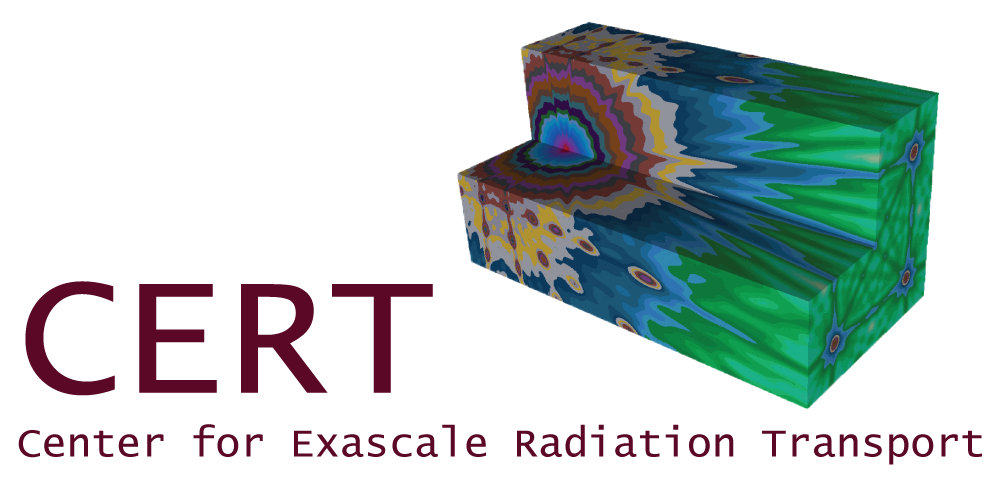
\includegraphics[width=0.25\textwidth]{cert_logo_maroon.png}
     \end{figure}
    \end{block}
    %%%%%%%%%%%%%%%%%%%%%%%%%%%%%%%%%%%%%%%%%%%%%%%%%
}
\end{minipage}
\end{beamercolorbox}
\end{column}

\end{columns}
\end{frame}
\end{document}

    %%%%%%%%%%%%%%%%%%%%%%%%%%%%%%%%%%%%%%%%%%%%%%%%%
    %\begin{block}{The transport equation}
    %\vspace{-16mm}
    %    \begin{align*}
    %    \small
    %    \om \cdot \nabla \psi(\vec{r}, E, \om) + \Sigma_t(\vec{r}, E) \psi(\vec{r}, E, \om) &= \frac{1}{4 \pi} \int_0^\infty \ud{E'} \Sigma_{s}(\vec{r}, E' \rightarrow E) \phi (\vec{r}, E') \;+ \nonumber \\
    %     &\qquad \frac{\chi(\vec{r}, E) }{4 \pi \, \keff} \int_0^\infty \ud{E'} \nu \Sigma_{f}(\vec{r}, E') \phi (\vec{r}, E')
    %    \end{align*}
    %    {
    %\footnotesize
    %With $\vec{r}$ the spatial coordinate, $E$ the energy, $\om$ the direction of travel, $\psi$ the radiation angular intensity, $\Sigma_t$ the total cross section, $\Sigma_s$ the scattering cross section, $\nu\Sigma_f$ the neutron production by fission cross section, $\keff$ the criticality eigenvalue, $\chi$ the fission distribution, and $\phi$ the scalar (angle-integrated) flux.
    %}
    %\end{block}
    %\vfill
